\renewcommand*\descriptionlabel[1]{\hspace\leftmargin$#1$}
\setcounter{tocdepth}{5}
\setcounter{secnumdepth}{5}


\section{Depletion Step Mesh Refinement}

As previously shown, there are many different methods available for modeling the online reprocessing of molten salt reactors. Previously, Rykhlevskii has generated results for the molten salt breeder reactor using the bulk batchwise method. This method is primarily useful due to the straightforward nature of its implementation. However, it is less accurate and more costly than other methods. The other batchwise method, steady batch, has approximately the same computational cost, but provides more accuracy by making better use of each depletion step available.

The continuous methods are all the same in terms of computational cost. The main difference is in the interpretation used when provided with the cycle time data. Because the cycle times given are the amount of time to remove 100\% of a target, and the continuous methods all use exponential terms, different strategies are used. The most straightforward method is Direct Linear, while the methods of Cycle Rate and Cycle Time Decay are based on assumptions.

Though the different methods have been discussed in theory, it is more enlightening to view a practical application of each in order to compare them. In order to compare the different reprocessing methods more clearly, each is first taken through a mesh refinement study in order to determine the effects of depletion step. Intuitively, it is expected that the batchwise methods will perform exceedingly poorly with increasing depletion step size because of two main reasons. Firstly, less frequent depletion steps means the cross section and flux data is not updated as the fuel is depleted, leading to a less accurate results. However, this reason is shared by continuous reprocessing as well. The second reason is due to the less frequent application of reprocessing on a process which is intended to be occurring continuously.

This second reason can be more intuitively understood with an example. Consider a simple thermal-spectrum system where uranium is fissioning and reprocessing is taking place. If xenon is physically continuously reprocessed, then the total absorption by xenon is reduced. However, using a longer batchwise step size results in xenon forming and capturing neutrons. Only after the depletion step size time elapses is batchwise reprocessing performed and the xenon is removed. By this point, many neutrons have already been captured, affecting reactor performance.

\subsection{Batchwise Reprocessing}

\subsubsection{Bulk Batchwise}

A depletion step mesh refinement study using the bulk batchwise reprocessing version of SaltProc was performed by Rykhlevskii comparing 3, 6, 12, and 24 day depletion steps over 25 years for the Transatomic Power Molten Salt Reactor \cite{rykhlevskii_fuel_2020}. Because the bulk batchwise method has already been analyzed and discussed, results for that method will not be separately generated here. The bulk batchwise model of the MSBR by Rykhlevskii will be used as an item of comparison to the continuous and steady batchwise methods implemented in this work \cite{rykhlevskii_advanced_2018}.

\subsubsection{Steady Batchwise}

Based on this previous work, this work instead checks 1, 1.5, 3, and 6 day depletion steps for the steady batchwise reprocessing method which is now used in SaltProc. This is to check if a smaller step size than 3 days should be implemented, or if the accuracy gained is not worth the increased computational cost. Previously, Rykhlevskii used a 3 day depletion step in the bulk batchwise analysis of the MSBR over 20 years \cite{rykhlevskii_advanced_2018}. Considering the computational cost increases associated with using a smaller depletion step size, this depletion step size selection was well made. Therefore, for the longer net depletion time results, the 3 day depletion step will also be used. However, it is still beneficial to check how the 3 day depletion step results would compare to longer and shorter depletion times.

Although the cycle time was previously implemented as 100\% removal, the krypton and xenon removal is instead around 91\%. This is because of the different liquid phase mass transfer coefficient, and was discussed by Rykhlevskii previously \cite{rykhlevskii_fuel_2020}. For the other elements, a fixed value is assumed. One difference this has is that instead of having a mass of zero in the xenon-135 and xenon-136 figures, there will be plot showing how the xenon concentrations vary over time. Additionally, the protactinium removal is 9.5\% instead of 95\% every three days, which results in a shift in the average feed rates which were determined in the bulk batchwise SaltProc solution.

\paragraph{Effects of Reprocessing}

Figures \ref{fig:steady-batch-k} through \ref{fig:steady-batch-xe136} show how the different depletion step sizes impact the effective multiplication factor and concentration of different isotopes in the system after reprocessing has occurred.

It can be seen by the evolution of the effective multiplication factor that different steady state values are being approached. The difference after 24 days between the 1 day depletion step and 6 day depletion step is roughly 656 pcm, 490 pcm for the 1 and 3 day steps, and 260 pcm for the 1 and 1.5 day steps. Based on the trend shown, it is expected for these values to only diverge further apart over time.

\begin{figure}[H]
  \centering
  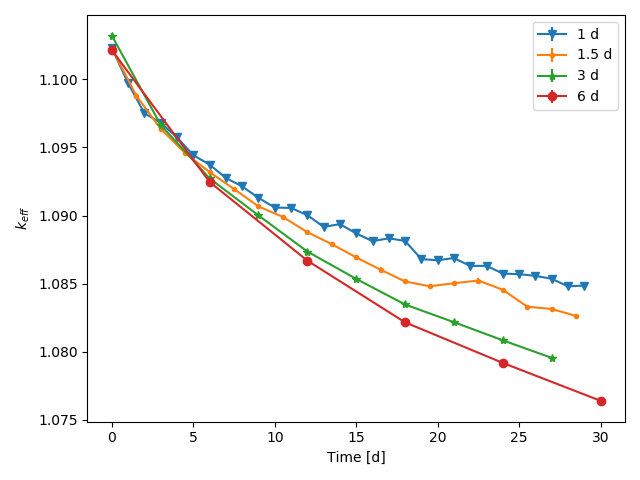
\includegraphics[scale=0.5]{images/keff-batch-dep-refine.png}
  \caption{k$_{eff}$ over time using various depletion step sizes with steady batchwise reprocessing.}
   \label{fig:steady-batch-k}
\end{figure}

A similar trend of approaching a different steady state value can be seen from the thorium-232 and uranium-233 masses over time. After 30 days, the thorium-232 maximum difference is roughly 22 kilograms between the 1 day and 6 day depletion steps. The uranium-233 difference is roughly 13 kg, which is a slightly smaller difference than the thorium-232. The reason the longer time step has a reduced thorium-232 and uranium-233 mass is because they are both treated as feed rates which maintain a constant net mass for the system. Because the reprocessing is less frequent, there are more parasitic absorbers built up in the core, reducing the total amount of material which is burned. Therefore, there is a smaller feed rate provided to the system.

\begin{figure}[H]
  \centering
  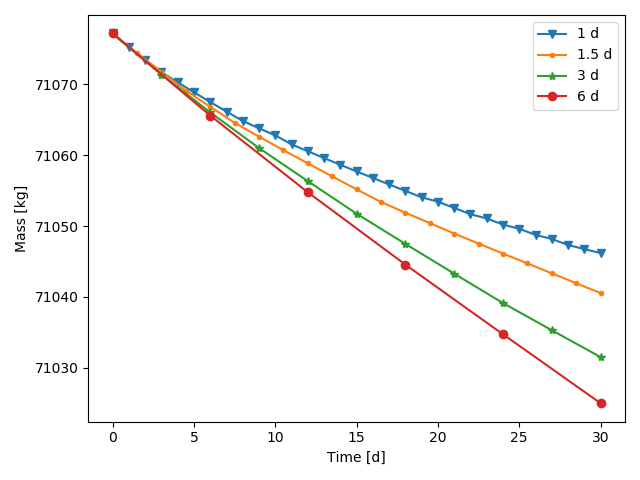
\includegraphics[scale=0.5]{images/Th232_sp_comp.png}
  \caption{Thorium-232 mass over time using various depletion step sizes with steady batchwise reprocessing.}
   \label{fig:steady-batch-th}
\end{figure}

\begin{figure}[H]
  \centering
  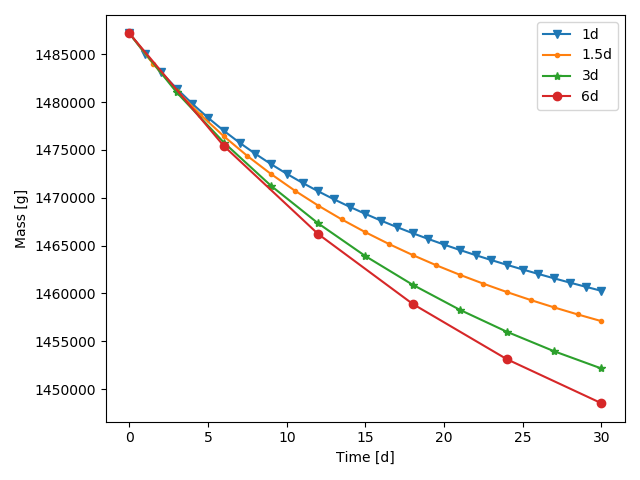
\includegraphics[scale=0.5]{images/U233_sp_comp.png}
  \caption{Uranium-233 mass over time using various depletion step sizes with steady batchwise reprocessing.}
   \label{fig:steady-batch-u}
\end{figure}

Because xenon-135 has a very high thermal neutron absorption cross section, it is useful to see how its mass varies. It can be seen that it is at a steady state value which is the same for each of the different depletion step sizes. Previously, it was shown that the relative error should scale based on the depletion step size, yet these values are the same. The reason for this is because the cycle time of xenon in the system is 20 seconds, while the smallest depletion step size is significantly larger than that. This results in a situation where the mass of xenon-135 builds up, stabilizes, and is reprocessed. In order to view the actual steady state of xenon-135 for the cycle time of 20 seconds, a depletion step size would have to be on the order of seconds instead of days.

\begin{figure}[H]
  \centering
  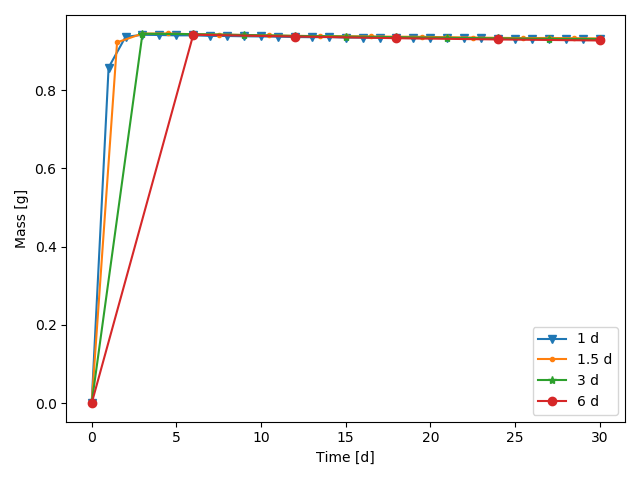
\includegraphics[scale=0.5]{images/Xe135_sp_comp.png}
  \caption{Xenon-135 mass over time using various depletion step sizes with steady batchwise reprocessing.}
   \label{fig:steady-batch-xe135}
\end{figure}

After xenon-135 absorbs a neutron, it can form xenon-136. By monitoring the concentration of xenon-136 in the system, the amount of xenon-135 which has parasitic absorptions can be understood more clearly, as there is a directly proportional relationship. Figure \ref{fig:steady-batch-xe136} shows how this concentration varies over time, which can clearly show the difference between the depletion step sizes. The steady state concentration of xenon-136, which directly correlates to the amount of parasitic absorption by xenon-135, directly correlates to the depletion step size. The ratio of depletion step sizes is somewhat close to the ratio of the steady state concentrations, with the ratio of 1.5, 3, and 6 day depletion steps to the 1 day depletion steps being 1.53, 3.1, and 6.3, respectively.

\begin{figure}[H]
  \centering
  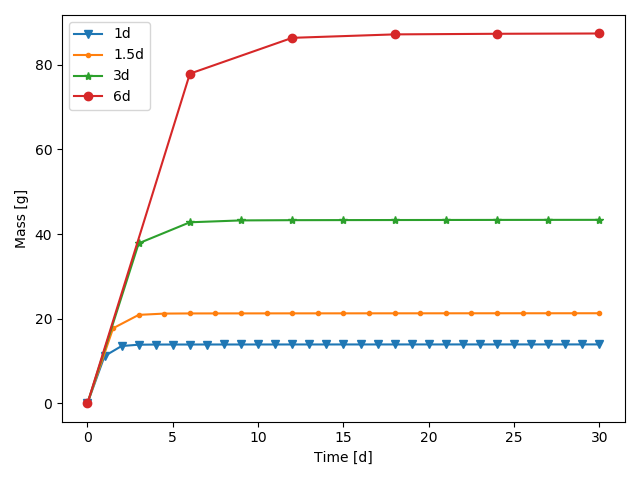
\includegraphics[scale=0.5]{images/Xe136_sp_comp.png}
  \caption{Xenon-136 mass over time using various depletion step sizes with steady batchwise reprocessing.}
   \label{fig:steady-batch-xe136}
\end{figure}

\paragraph{Feed and Removal Rates}

Figures \ref{fig:steady-batch-th-repr} and \ref{fig:steady-batch-u-repr} show the feed rates of thorium-232 and uranium-233, respectively. As previously discussed, the overall feed rate has the objective of maintaining constant mass. This explains why the feed rate for longer depletion steps is smaller than the feed rates associated with shorter depletion steps, as the reprocessing is less frequent, leaving more parasitic absorbers in the core. 

\begin{figure}[H]
  \centering
  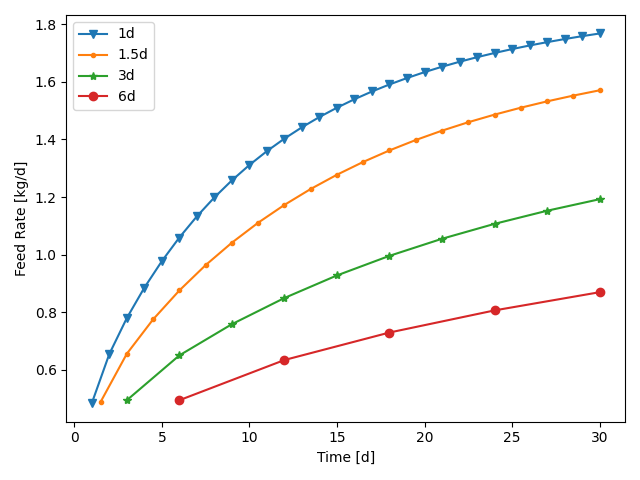
\includegraphics[scale=0.5]{images/feed_Th232_6d_sp_comp.png}
  \caption{Thorium-232 feed rate over time using various depletion step sizes with steady batchwise reprocessing.}
   \label{fig:steady-batch-th-repr}
\end{figure}

\begin{figure}[H]
  \centering
  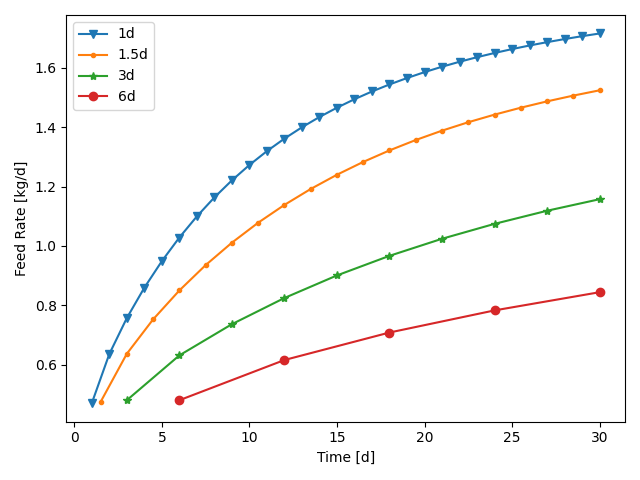
\includegraphics[scale=0.5]{images/feed_U233_6d_sp_comp.png}
  \caption{Uranium-233 feed rate over time using various depletion step sizes with steady batchwise reprocessing.}
   \label{fig:steady-batch-u-repr}
\end{figure}

Figures \ref{fig:steady-batch-xe135-repr} and \ref{fig:steady-batch-xe136-repr} show the removal rates of xenon-135 and xenon-136, respectively. The xenon-136 removal rate is fairly straightforward to understand, as it was previously shown that the steady state concentration of xenon-136 is higher for the longer depletion step sizes. This means that the removal rate would also need to be higher, since the amount removed is proportional to the amount present in the system. For the xenon-135, the removal rate relationship may not immediately be clear since the steady state mass of xenon-135 after reprocessing is the same for the different depletion step sizes. However, the removal rate is higher for the shorter depletion step size because the xenon-135 builds up to a steady state value before reprocessing occurs. This means that every time reprocessing occurs, roughly the same amount of xenon-135 is removed. Thus, more frequent reprocessing yields an increased removal rate.

\begin{figure}[H]
  \centering
  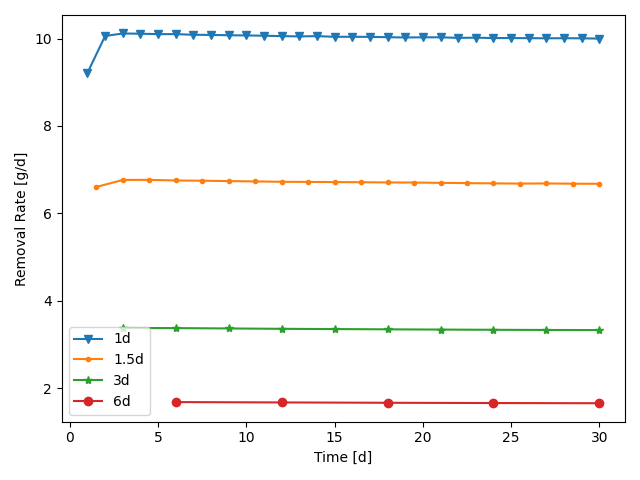
\includegraphics[scale=0.5]{images/waste_Xe135_6d_sp_comp.png}
  \caption{Xenon-135 removal rate over time using various depletion step sizes with steady batchwise reprocessing.}
   \label{fig:steady-batch-xe135-repr}
\end{figure}

\begin{figure}[H]
  \centering
  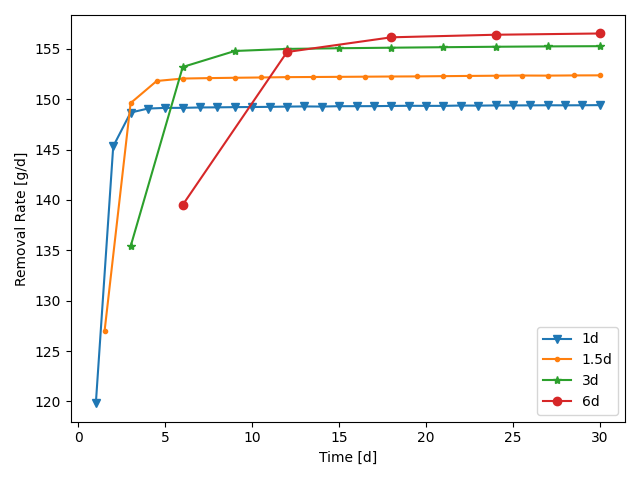
\includegraphics[scale=0.5]{images/waste_Xe136_6d_sp_comp.png}
  \caption{Xenon-136 removal rate over time using various depletion step sizes with steady batchwise reprocessing.}
   \label{fig:steady-batch-xe136-repr}
\end{figure}

\subsection{Continuous Reprocessing}

For the batchwise methods, depletion time steps beyond 6 days are not considered. This is because a larger time step causes more error, and it can be seen that the difference between the 6 day depletion step and the smaller depletion steps is non-negligible.

For the continuous methods, the error buildup from using larger depletion steps is purely due to not updating various simulation data rather than from lack of updating the material compositions based on reprocessing. Due to this, larger time steps can be considered. In order to determine the impact of the updated simulation data, initially chosen depletion time steps of 1, 3, 6, 15, and 30 days are implemented. Additionally, although different continuous methods have been introduced, the depletion step mesh refinement only needs to consider one of the methods. This is because the continuous methods used all have the same general form and only alter the specific reprocessing constants implemented. Thus, the direct linear method is selected to determine the optimal depletion step size for the continuous methods. Additionally, it has been used in several other works and is very similar to the Cycle Rate method \cite{xia_development_2019, nuttin_potential_2005, zhou_fuel_2018}.

\subsubsection{Smaller Depletion Steps}

The results from using depletion steps of 1, 3, 6, 15, and 30 days can be seen in Figures \ref{fig:DL-cont-k} through \ref{fig:DL-cont-xe136}. The results regarding the effective multiplication factor show that, after 30 days, all of the effective multiplication factors are within stochastic error of each other. 

\begin{figure}[H]
  \centering
  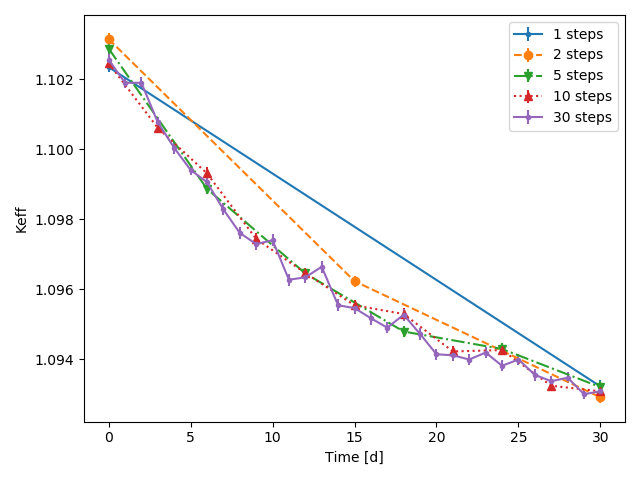
\includegraphics[scale=0.5]{images/DL_NSTEP_keff.png}
  \caption{k$_{eff}$ over time using various depletion step sizes with direct linear continuous reprocessing.}
   \label{fig:DL-cont-k}
\end{figure}

For the thorium-232 and uranium-233 masses, the values align within fractions of a percent of each other after 30 days of depletion. Additionally, it can be seen that there are sudden jumps in the thorium-232 mass. This is because of rounding which occurs due to a limit to the precision of the data which is available from Serpent2.

\begin{figure}[H]
  \centering
  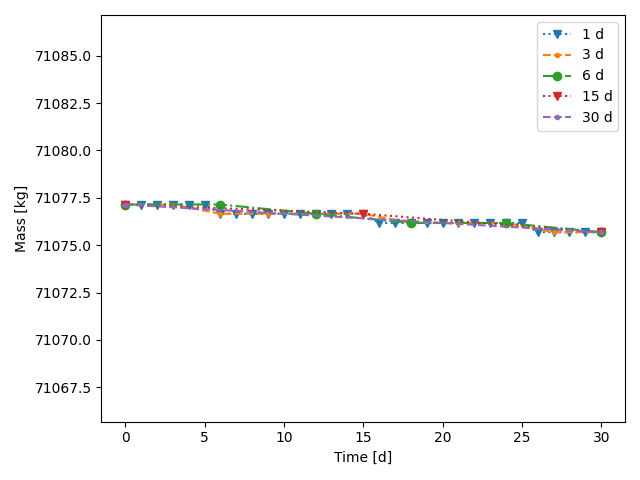
\includegraphics[scale=0.5]{images/DL_NSTEP_Th-232_mass.png}
  \caption{Thorium-232 mass over time using various depletion step sizes with direct linear continuous reprocessing.}
   \label{fig:DL-cont-th}
\end{figure}

\begin{figure}[H]
  \centering
  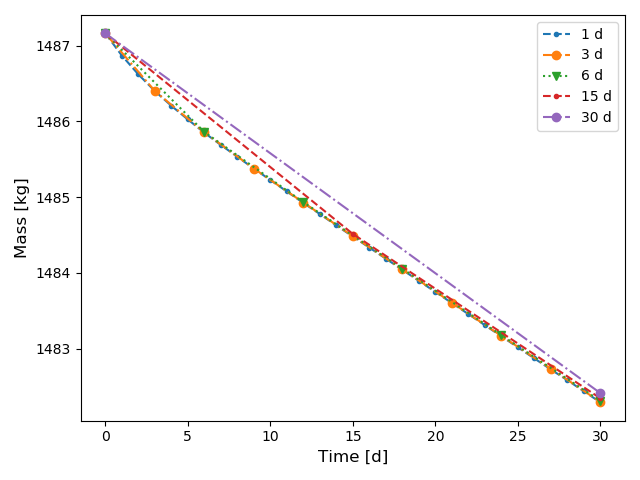
\includegraphics[scale=0.5]{images/DL_NSTEP_U-233_mass.png}
  \caption{Uranium-233 mass over time using various depletion step sizes with direct linear continuous reprocessing.}
   \label{fig:DL-cont-u}
\end{figure}

The xenon-135 steady state mass is the same for each of the different step sizes, which is expected. Additionally, the xenon-136 steady state mass is also the same for the different depletion step sizes, showing that the capture rate of the xenon-135 does not vary significantly even when adjusting the depletion step size from 1 day to 30 days.

\begin{figure}[H]
  \centering
  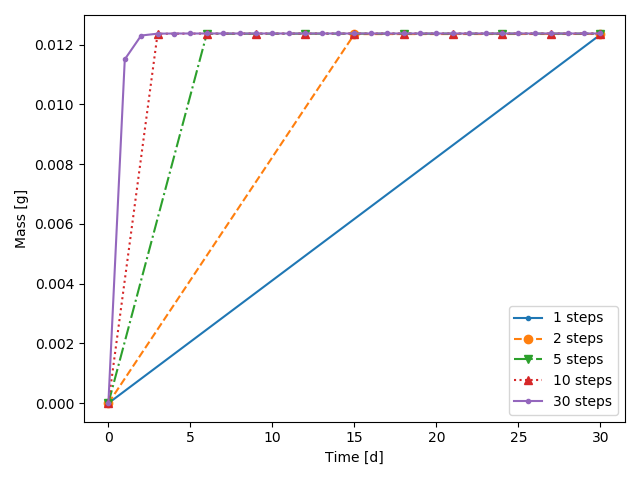
\includegraphics[scale=0.5]{images/DL_NSTEP_Xe-135_mass.png}
  \caption{Xenon-135 mass over time using various depletion step sizes with direct linear continuous reprocessing.}
   \label{fig:DL-cont-xe135}
\end{figure}

\begin{figure}[H]
  \centering
  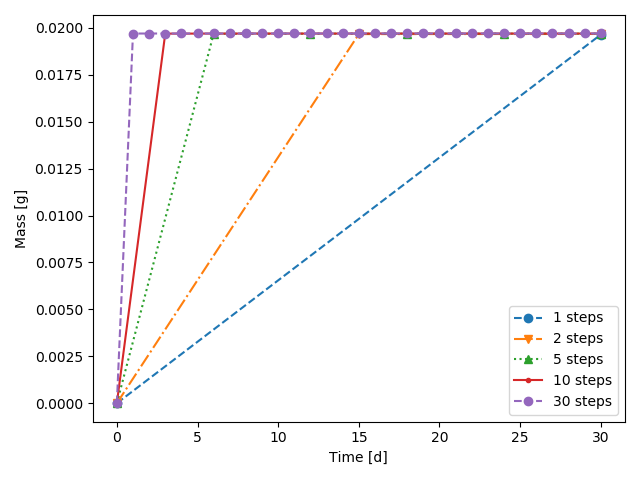
\includegraphics[scale=0.5]{images/DL_NSTEP_Xe-136_mass.png}
  \caption{Xenon-136 mass over time using various depletion step sizes with direct linear continuous reprocessing.}
   \label{fig:DL-cont-xe136}
\end{figure}

Because these results are all very close to each other, it is prudent to test for larger depletion step sizes in order to determine how much computational cost reduction can be afforded while maintaining high accuracy in the results.

\subsubsection{Larger Depletion Steps}

The next set of depletion step sizes selected are 30, 60, 120, and 360 days. The smallest step size, 30 days, is selected in order to properly compare the larger depletion step sizes with a step size which has been shown to give results which are very close to those of a 1 day depletion step size. The results can be seen in Figures \ref{fig:DL-cont-k-2} through \ref{fig:DL-cont-xe136-2}. 

\begin{figure}[H]
  \centering
  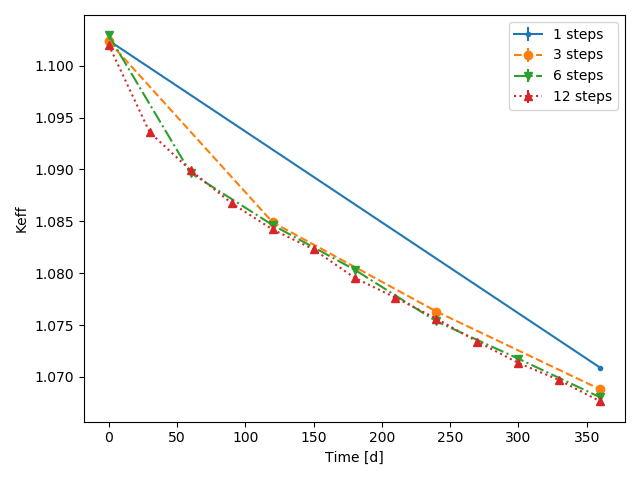
\includegraphics[scale=0.5]{images/DL_NSTEP_keff-large.png}
  \caption{k$_{eff}$ over time using various depletion step sizes with direct linear continuous reprocessing.}
   \label{fig:DL-cont-k-2}
\end{figure}

The 60 day depletion time effective multiplication factor at 360 days is not within stochastic error of the value for the 30 day depletion time. The error bounds are only 5 pcm apart, but since the computational cost decrease is only a factor of two, the 30 day depletion step size is sufficiently large for the cases implemented in this work while maintaining a high level of precision and are used as the default when not specified.

The thorium-232 and uranium-233 masses follow a similar trend where the larger depletion step size has a higher mass of both isotopes. The difference in thorium can be seen by visualizing how the larger step sizes operate similarly to a tangent line from the shorter depletion step sizes. This is because the cross section and spectral data is not updated, and so the same rate of decrease is used over the entire depletion step. Because the system starts at beginning of cycle, the thorium is not yet in steady state and more is burned than added, so the decrease is expected. 

\begin{figure}[H]
  \centering
  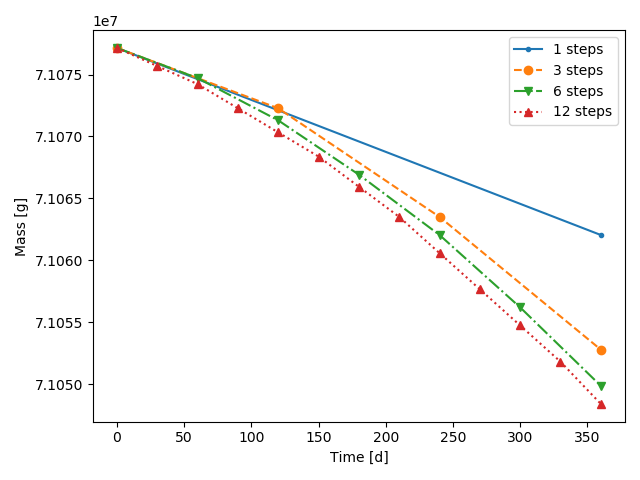
\includegraphics[scale=0.5]{images/DL_NSTEP_Th-232_mass-large.png}
  \caption{Thorium-232 mass over time using various depletion step sizes with direct linear continuous reprocessing.}
   \label{fig:DL-cont-th-2}
\end{figure}

For the uranium-233, a similar trend can be seen, though it is less pronounced. The main difference with thorium-232 is the fact that the thorium mass changes due to feed and neutron absorption, whereas the uranium-233 has feed, neutron absorption, and accumulation from the decay chain of the thorium-232 absorption. With this in mind, the difference of the uranium-232 and thorium-233 figures becomes more clear. For the shorter depletion steps, a similar trend as in the thorium-232 occurs where the rate is matches for the depletion step. However, the thorium-232 is also a factor, and since the thorium-232 has a greater mass for larger depletion step sizes, this results in more uranium-232 being bred as well.

\begin{figure}[H]
  \centering
  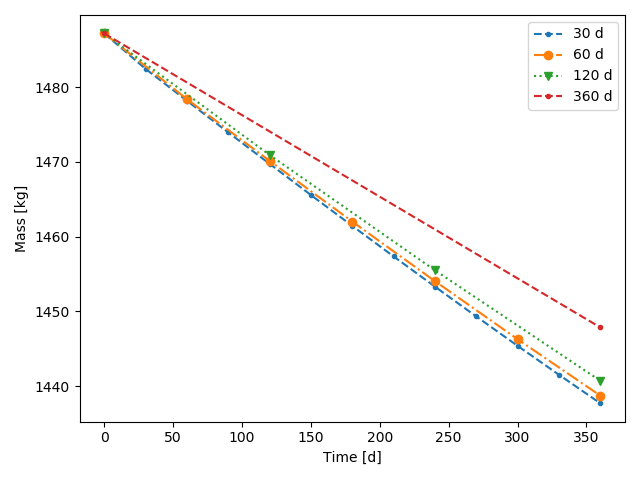
\includegraphics[scale=0.5]{images/DL_NSTEP_U-233_mass-large.png}
  \caption{Uranium-233 mass over time using various depletion step sizes with direct linear continuous reprocessing.}
   \label{fig:DL-cont-u-2}
\end{figure}

The xenon-135 and xenon-136 masses match closely, with differences on the order of milligrams. This agrees well with the previous results generated as well. The reason the results agree well is because the xenon-135 concentration is expected to approach a constant result with increasing flux. This is because the xenon-135 comes from the decay of iodine-135, which scales proportionally to the flux. However, the xenon-135 has a large capture cross section, and is altered into xenon-136 proportionally to the flux as well. This shows why there is not a large difference even though there is a difference of 324 pcm between the effective multiplication factors of the 360 and 30 day depletion step sizes.

\begin{figure}[H]
  \centering
  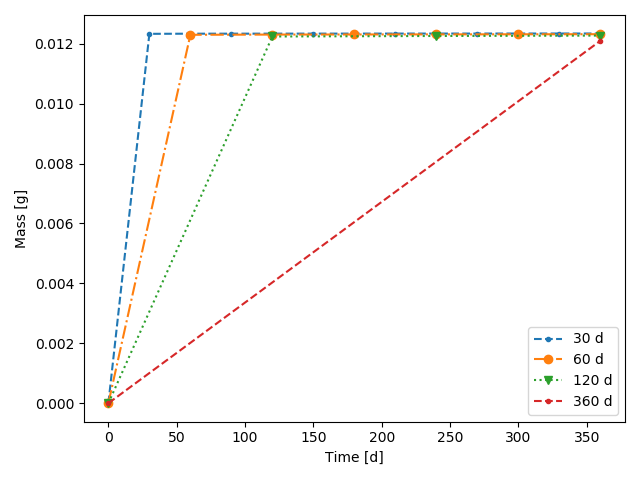
\includegraphics[scale=0.5]{images/DL_NSTEP_Xe-135_mass-large.png}
  \caption{Xenon-135 mass over time using various depletion step sizes with direct linear continuous reprocessing.}
   \label{fig:DL-cont-xe135-2}
\end{figure}

The xenon-136 is also captured with a rate proportional to the flux, though the capture cross section is significantly lower than that of xenon-135 for the thermal spectrum used in the MSBR. This can be seen in the mass of xenon-136, which has a higher steady state concentration that that of xenon-135. The main limiting factor on both of these xenon isotopes is the reprocessing term, which keeps the steady state mass of both much smaller than they would be without the reprocessing.

\begin{figure}[H]
  \centering
  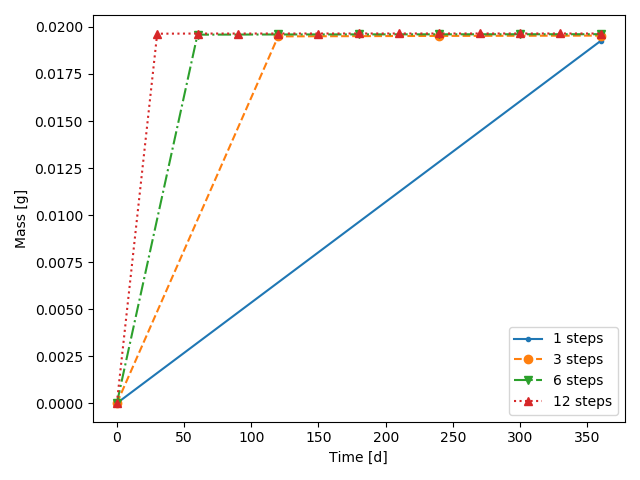
\includegraphics[scale=0.5]{images/DL_NSTEP_Xe-136_mass-large.png}
  \caption{Xenon-136 mass over time using various depletion step sizes with direct linear continuous reprocessing.}
   \label{fig:DL-cont-xe136-2}
\end{figure}


\subsection{Variable Depletion Step Size}

Previously, the depletion step size needed for a reasonably converged result was investigated using a constant depletion step size. However, it is understood that the reactor will experience some rapid initial changes, after which the changes slow and eventually the reactor reaches steady state. Therefore, it is reasonable to expect that in the early times, small depletion step sizes should be used, while at later times, larger depletion step sizes should be used.

Because it was previously shown for continuous reprocessing that the depletion step sizes smaller than 30 days give results within stochastic error for the effective multiplication factor, the 30 day depletion step size will be the smallest considered step size. Several cases are considered over a net depletion time of 360 days in order to determine the effects of varying the depletion step size at various points in the simulation. Case A uses 12 30 day steps; Case B uses 6 30 day steps and 1 180 day step; Case C uses 3 30 day steps, 1 90 day step, and 1 180 day step; Case D uses 1 30 day step and 1 330 day step; Case E uses 1 180 day step and 6 30 day steps; and Case F uses 1 360 day step. The results for each case at the time value of 360 days are given in Table \ref{tab:var-dep-step-size}.


\begin{table}[H]
\renewcommand{\arraystretch}{1.25}
\caption{Variable Depletion Step Size Results}
\label{tab:var-dep-step-size}
\begin{center}
\begin{tabular}{ | c | c | c | c | }
 \hline
 Case & $k_{eff}$ & $\Delta k_{eff}$ [pcm]  & Simulations\\
 \hline
 \hline
 A & 1.06801 $\pm$ 0.00017  & - & 12\\
 B & 1.06844 $\pm$ 0.00015 & 43 $\pm$ 32  & 7\\
 C & 1.06857 $\pm$ 0.00016  & 56 $\pm$ 33  & 5\\
 D & 1.07034 $\pm$ 0.00016 & 233 $\pm$ 33  & 2\\
 E & 1.06846 $\pm$ 0.00016 & 45 $\pm$ 33  & 7\\
 F & 1.07071 $\pm$ 0.00017 & 270 $\pm$ 34 & 1\\
 \hline
\end{tabular}
\end{center}
\end{table}

%\begin{table}[H]
%\renewcommand{\arraystretch}{1.25}
%\caption{Varyiable Depletion Step Size Results}
%\label{tab:var-dep-step-size}
%\begin{center}
%\begin{tabular}{ | c | c | c | c | c | c | }
% \hline
% Case & $k_{eff}$ & $\Delta k_{eff}$ [pcm] & $Th_{232}$ [Mg] & $U_{233}$ [Mg] & Simulations\\
% \hline
% \hline
% A & 1.06801 $\pm$ 0.00017  & - & 71.05 & 1.44 & 12\\
% B & 1.06844 $\pm$ 0.00015 & 43 $\pm$ 32 & 71.05 & 1.44 & 7\\
% C & 1.06857 $\pm$ 0.00016  & 56 $\pm$ 33 & 71.05 & 1.44 & 5\\
% D & 1.07034 $\pm$ 0.00016 & 233 $\pm$ 33 & 71.06 & 1.45 & 2\\
% E & 1.06846 $\pm$ 0.00016 & 45 $\pm$ 33 & 71.05 & 1.44 & 7\\
% F & 1.07071 $\pm$ 0.00017 & 270 $\pm$ 34 & 71.06 & 1.45 & 1\\
% \hline
%\end{tabular}
%\end{center}
%\end{table}

%From the thorium-232 and uranium-233 mass results, it can be seen Cases D and F are outliers. The trait in common with these two runs is the largest depletion step size implemented, as both of these runs have larger depletion step sizes than any of the other runs, resulting in far fewer simulations performed.

For the result of the effective multiplication factor, the difference from Case A was taken for the rest of the cases. These results show that Cases B, C, and E are all very close to Case A. Cases D and E are the outliers, which is also reflected in the number of simulations run. Case D uses a short depletion time step initially followed by a single long step, which should have allowed for the simulation data to update based on the presence of fission products which were not initially present.
However, this impact is likely offset by the continuous reprocessing, resulting in more impact purely due to the general changes in the system. It seems that multiple steps are needed during the first 360 days of operation in order to properly account for the changes within the reactor, such as Case E, which leads with a depletion step size of 180 days but then proceeds to follow it with six 30 day depletion steps.

The variable depletion step size could be considered to have an impact if the reactor were at steady-state, but after only 360 days of operation, there are still changes occurring \cite{rykhlevskii_advanced_2018}. This is the reason why having more simulations yielded better results than the cases which had fewer simulations.

\subsection{Computational Cost Analysis}

In order to provide a useful measure of computational cost, Table \ref{tab:comp-cost-methods-1} is generated. This table represents the compuational cost of forming the depletion step mesh refinement study in the units of "number of simulations required," as this is the largest impact on run time. The depletion step size used by the batchwise methods is 3 days, while the continuous method uses 30 day depletion steps.

The cost for SaltProc based batchwise methods can be calculated by first accounting for all internal depletion times. These all require 2 simulations when run using Serpent2, as the pre-reprocessed simulation is also run. An optimized batchwise method could remove the double running, which would significantly reduce computational cost. Additionally, as can be seen in the forumla for calculating the cost, reduction can be achieved by maximizing the depletion step size or reducing the net depletion time, or $T_{net}$.

\begin{table}[H]
\renewcommand{\arraystretch}{1.25}
\caption{Computation Cost Using Constant Depletion Steps}
\label{tab:comp-cost-methods-1}
\begin{center}
\begin{tabular}{ | c | c | c | c | c | }
 \hline
 Method & Cost Formula & 30 days & 1 year & 10 years\\
 \hline
 \hline
 SaltProc Batchwise & $2 T_{net} \Delta t^{-1}$ & 20 & 244 & 2435\\
 Optimized Batchwise & $T_{net} \Delta t^{-1} + 1$ & 11 & 123 & 1219\\
 Continuous (All) & $T_{net} \Delta t^{-1} + 1$ & 2 & 14 & 123\\
 \hline
\end{tabular}
\end{center}
\end{table}

Because continuous reprocessing enables the use of depletion time steps on the order of 10x larger while retaining a similar level of precision, the computational cost is significiantly lowerer than the batchwise computational cost.

\section{Advanced Protactinium Decay Model}

The original method used by Rykhlevskii to model the decay of protactinium-233 into uranium-233 was to feed a mass of uranium-233 into the core equivalent to the mass of protactinium-233 pumped out every 3 days \cite{rykhlevskii_advanced_2018}. With the implementation of continuous reprocessing methods, the breeding can be more accurately modeled. In the new method, protactinium-233 is continuously removed and allowed to decay. Once it decays, the uranium-233 is then continuously added back into the core.

It is expected for the largest impact to be at beginning of cycle, while at steady state this improved method will likely have only a minor effect on the results. The results of this analysis can be seen in Figures \ref{fig:DL-cont-k-adv} through \ref{fig:DL-cont-xe136-adv}, where the continuous method implemented for both was the Direct Linear method, and 305 day depletion steps were used over a period of 3660 days, or roughly ten years. Although this depletion step size is larger than those previously used, it is expected to still give reasonable accurate results. Additionally, the discard and salt discard processes are not considered here, as only the differences between the different feed rate methods are being investigated.

The effective multiplication factor for the realistic uranium-233 feed approach can be seen to drop rapidly, and then begin leveling off after around 3 years. The reason for this difference in behaviour is because the feed which uses the SaltProc averaged value makes a steady state assumption, which allows for a full supply of uranium-233 available for feeding the reactor at all times. In can be seen that the slopes of the two different methods are beginning to converge slowly after a few year, and it is expected that they would eventually match. However, if the batch discard processes are included, a true steady state equilibrium would not be reached, resulting in at least some minor differences between the methods.

\begin{figure}[H]
  \centering
  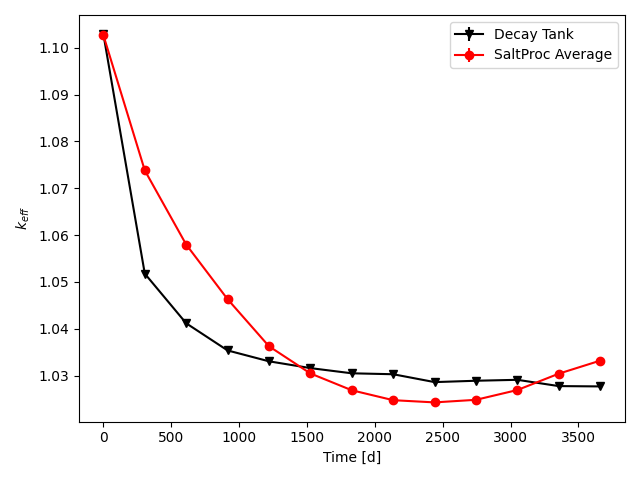
\includegraphics[scale=0.5]{images/adv-keff.png}
  \caption{k$_{eff}$ over time using various depletion step sizes with direct linear continuous reprocessing.}
   \label{fig:DL-cont-k-adv}
\end{figure}

The thorium-232 masses have a fairly constant difference from each other over the entire run. The reason for this is likely due to the fact that there is less uranium-233 being added to the system with the realistic approach, meaning more interactions with thorium-232 occur instead. This results in a lower effective multiplication factor, at least initially, which provides increased uranium-233 production, and lower thorium-232 mass.

\begin{figure}[H]
  \centering
  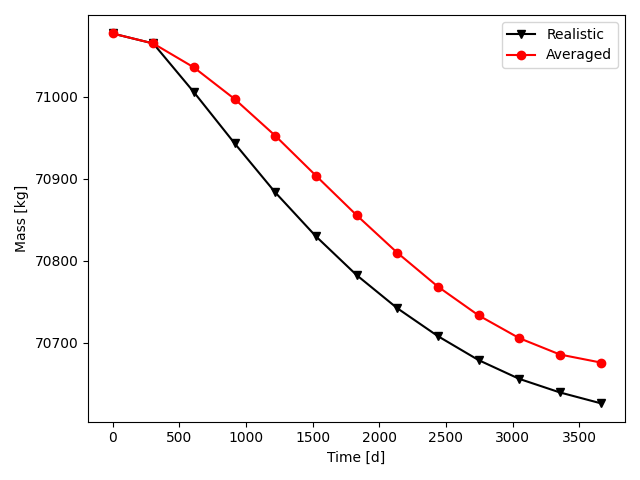
\includegraphics[scale=0.5]{images/adv-Th232.png}
  \caption{Thorium-232 mass over time using various depletion step sizes with direct linear continuous reprocessing.}
   \label{fig:DL-cont-th-adv}
\end{figure}

The uranium-233 for the realistic method follows a trend which is expected, which is a sharp initial drop followed by a decrease in the rate of change. After the sharp drop, the protactinium decay tank fills, and fresh uranium-233 is supplied to the system in an increasing quantity. For the averaged method, because the uranium-233 was burned at a higher rate, this leads to a decrease in the total amount. It is expected that there will be a few oscillations in the uranium-233 mass for the averaged system until it finally achieves a steady state value, though this is only true if the system only has continuous reprocessing processes. This oscillation is expected because initially, there is more uranium-233 which fissions, rapidly decreasing the quantity while maintaining a higher effective multiplication factor. This causes the uranium-233 to burn quickly, dropping the net mass until it reaches a point that the effective multiplication factor decreases while the uranium-233 mass is also lowered, reducing probability of fission as well as the number of neutrons. This allows the feed rate to build up more uranium-233 in the system, repeating the process.

\begin{figure}[H]
  \centering
  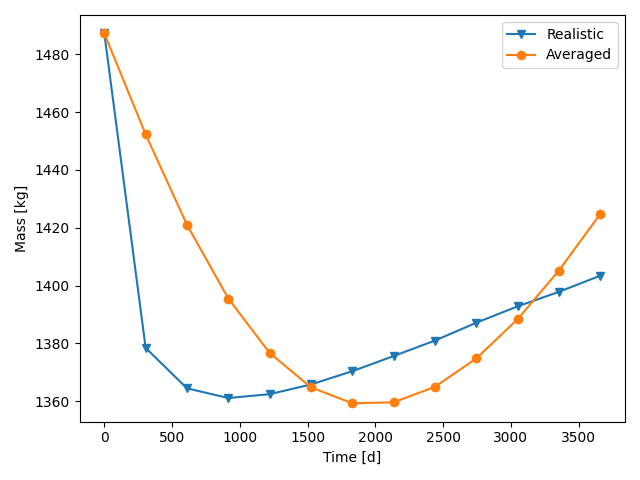
\includegraphics[scale=0.5]{images/adv-U233.png}
  \caption{Uranium-233 mass over time using various depletion step sizes with direct linear continuous reprocessing.}
   \label{fig:DL-cont-u-adv}
\end{figure}

For the xenon-135 and xenon-136, the masses are slightly smaller than the averaged method initially, which is due to the decreased uranium-233, resulting in fewer fission products being generated. However, after more time passes, the values match. This is due to the steady state value of xenon-135 not significantly changing when the flux is already large.

\begin{figure}[H]
  \centering
  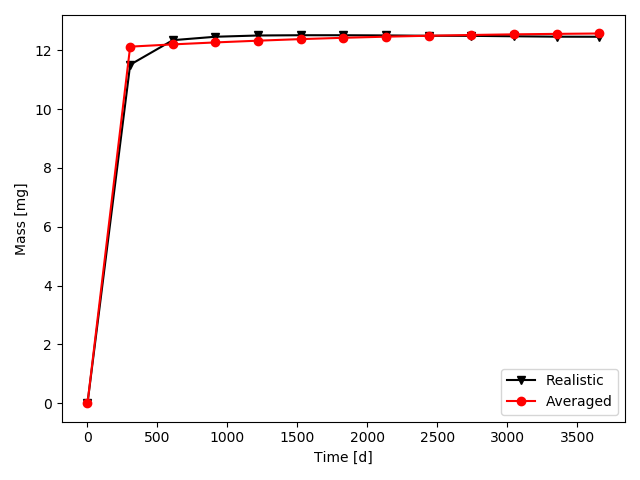
\includegraphics[scale=0.5]{images/adv-Xe135.png}
  \caption{Xenon-135 mass over time using various depletion step sizes with direct linear continuous reprocessing.}
   \label{fig:DL-cont-xe135-adv}
\end{figure}

\begin{figure}[H]
  \centering
  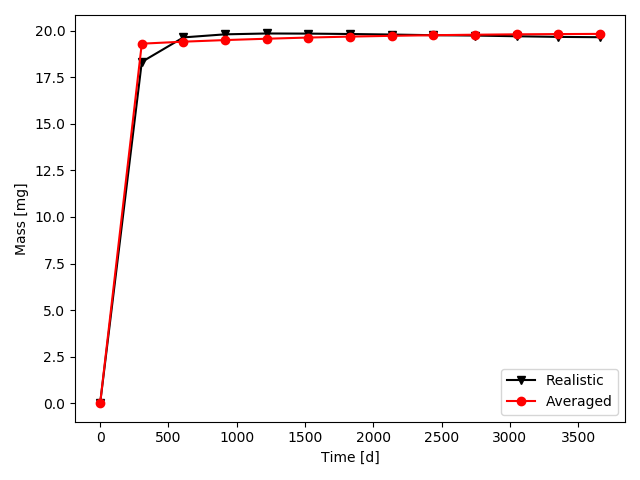
\includegraphics[scale=0.5]{images/adv-Xe136.png}
  \caption{Xenon-136 mass over time using various depletion step sizes with direct linear continuous reprocessing.}
   \label{fig:DL-cont-xe136-adv}
\end{figure}

\section{Comparisons of Methods}

There are many different works which have implemented batchwise reprocessing computational methods to simulate a continuous, online reprocessing scheme; many of which are discussed in the literature review. Thus, the question of how accurate these models are should be resolved. From previous work by Rykhlevskii as well as through the depletion step mesh refinement provided in this work, it has been shown that increasing the depletion step size causes batchwise methods to become less effective at simulating the physical, continuous process of online reprocessing \cite{rykhlevskii_fuel_2020}.

\subsection{Continuous Methods}

Although only the Direct Linear continuous reprocessing method has been used so far due to similarities between the continuous methods, it is still useful to determine how the different continuous methods compare in the MSBR.   For this comparison, the steady SaltProc-based averaged feed rates and modified cycle times are used as well as a 30 day depletion step size.


The effective multiplication factor, over the course of 360 days, has a difference on the order of 500pcm between the Cycle Time Decay, CTD, method and the Direct Linear and Cycle Rate, DL and CR, methods respectively. The Direct Linear and Cycle Rate methods are very close to each other, which is expected since the reprocessing constants are also very similar. The control method, CTRL, shows the effects of no reprocessing and no feed.

\begin{figure}[H]
  \centering
  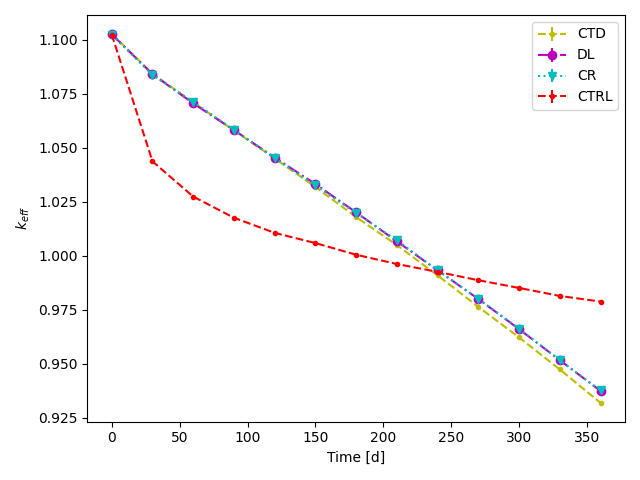
\includegraphics[scale=0.5]{images/cont-compare-keff-1.png}
  \caption{k$_{eff}$ over time comparing different continuous reprocessing methods.}
   \label{fig:continuous-compare}
\end{figure}

The reason the continuous methods shown here continue decreasing and are eventually overtaken by the control reprocessing is due to the protactinium reprocessing. Because the protactinium in these methods is continuously removed and the uranium-233 feed is averaged only over the first 90 days of the steady batchwise method, it is expected that the continuous model will become inaccurate some time after 90 days. This accuracy can be improved by implementing the advanced protactinium decay model which removes the dependency on an average uranium-233 feed rate.

However, the main purpose of this figure is to demonstrate how the different continuous methods compare to each other over a long period of time. Additionally, this figure shows how the effective multiplication factor without reprocessing drops below critical after roughly 300 days, and that having either a good estimate for the uranium-233 feed rate or a continuous method to generate the uranium-233 feed rate is very important for depletion modeling of the MSBR.


\subsection{Continuous and Batchwise Methods}

The continuous method selected for the comparison is the Direct Linear reprocessing method. For the batchwise methods, the bulk and steady batchwise reprocessing schemes from SaltProc early and current versions are used. For the bulk batchwise reprocessing, the cycle times from the Robertson report are followed \cite{robertson_conceptual_1971}. Additionally, the uranium-233 and thorium-232 feed rates in the continuous model use the values from the bulk batchwise results \cite{rykhlevskii_advanced_2018}.

For the steady batchwise comparison, the modified cycle times are used which include an efficiency term on the xenon, krypton, and protactinium reprocessing constants. For the continuous comparison, the average thorium-232 and uranium-233 feed rates are generated from the 90 day runs and are implemented.

For all of these comparisons, the Direct Linear reprocessing method uses the average feed rate of the given batchwise method and the cycle times from the Robertson report \cite{robertson_conceptual_1971}. The SaltProc Direct Linear reprocessing method, which is intended to be a continuous approximation of the batchwise reprocessing method, will match the reprocessing constants used in the given batchwise method.

If the results are sufficiently close, then it may be reasonable for a continous method to be implemented in place of a batchwise method when the reprocessing scheme calls for a physically batchwise processes. This would allow for reduced computational cost and potentially large depletion step sizes to be implemented. If the results are not close, then these results will provide information on how the difference in reprocessing methods can affect results.


\subsubsection{Continuous and Bulk Batchwise Methods}

In this comparison, there are three different methods considered. These methods are the continuous Direct Linear, DL, method, the continuous SaltProc Direct Linear, SPDL, method; and the bulk batchwise SaltProc method. Figure \ref{fig:bulk-comapre-keff} shows how the effective multiplication factor varies over time for these methods. It can be seen that there is a jump at around 50 days for the bulk SaltProc data, which is caused by removal of the rare earths, as shown in the MSBR reprocessing scheme \cite{robertson_conceptual_1971}. However, it is clear to see here that the continuous methods are not able to match the bulk batchwise reprocessing results very closely at all, even using the SaltProc Direct Linear method which attempts to replicate the same reprocessing constants.

\begin{figure}[H]
  \centering
  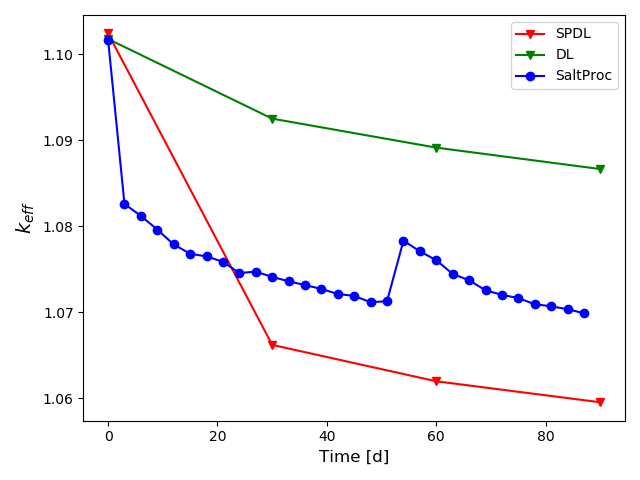
\includegraphics[scale=0.5]{images/soln-3-keff.png}
  \caption{k$_{eff}$ over time comparing bulk batchwise results to continuous methods.}
   \label{fig:bulk-comapre-keff}
\end{figure}

Figures \ref{fig:bulk-comapre-th232} and \ref{fig:bulk-comapre-u233} show the mass of thorium-232 and uranium-233 over time, respectively. Overall, the masses of both isotopes are within a few kilograms, and do not have a large impact on the differences between the methods. For example, the spike in thorium-232 mass at 50 days when the rare earths are removed does not have nearly as much impact as the removal of the rare earths does on reactor behaviour.

\begin{figure}[H]
  \centering
  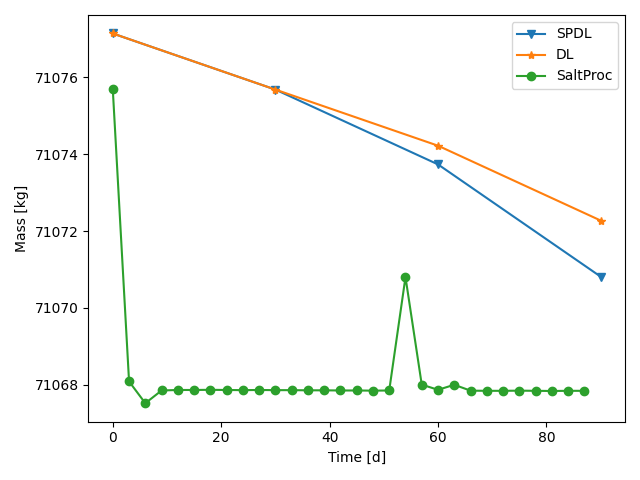
\includegraphics[scale=0.5]{images/soln-3-th232.png}
  \caption{Thorium-232 mass over time comparing bulk batchwise results to continuous methods.}
   \label{fig:bulk-comapre-th232}
\end{figure}

\begin{figure}[H]
  \centering
  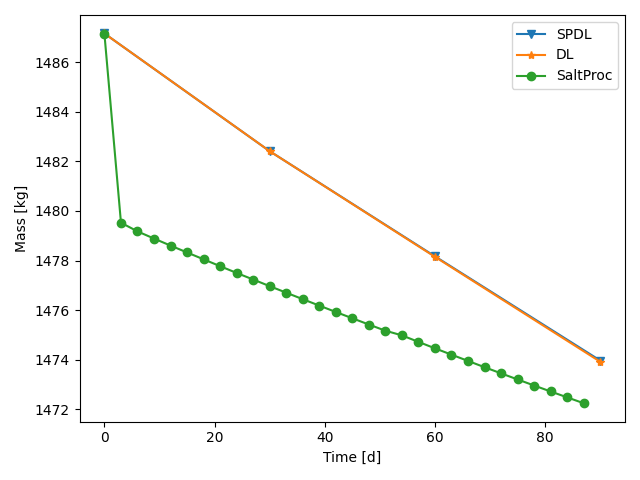
\includegraphics[scale=0.5]{images/soln-3-u233.png}
  \caption{Uranium-233 mass over time comparing bulk batchwise results to continuous methods.}
   \label{fig:bulk-comapre-u233}
\end{figure}

Figures \ref{fig:bulk-comapre-xe135} and \ref{fig:bulk-comapre-xe136} show how the xenon-135 and xenon-136 masses, respectively, change over time for the different methods. From these figures, it can be seen that the SPDL continuous method does a fairly good job of matching the bulk batchwise reprocessing method's masses. However, the SPDL method allows for slightly more fission product poisons to exist, such as xenon-135, which allows for more parasitic absorption, into isotopes such as xenon-136. This is the reason that the SPDL effective multiplication factor is lower than that of bulk SaltProc.

\begin{figure}[H]
  \centering
  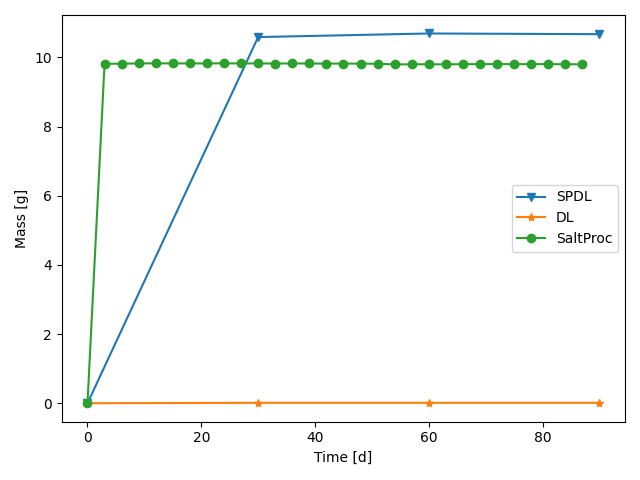
\includegraphics[scale=0.5]{images/soln-3-xe135.png}
  \caption{Xenon-135 mass over time comparing bulk batchwise results to continuous methods.}
   \label{fig:bulk-comapre-xe135}
\end{figure}

\begin{figure}[H]
  \centering
  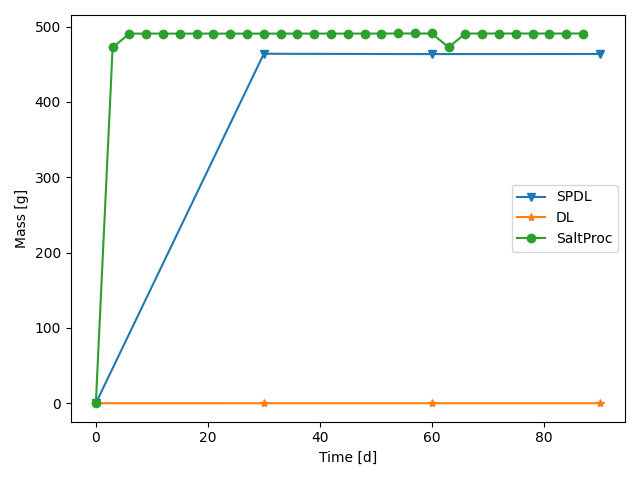
\includegraphics[scale=0.5]{images/soln-3-xe136.png}
  \caption{Xenon-136 mass over time comparing bulk batchwise results to continuous methods.}
   \label{fig:bulk-comapre-xe136}
\end{figure}

From these results, it can be concluded that using continuous reprocessing to perform a bulk reprocessing scheme will not yield same results. This also means that attempting to simulate a continuous reprocessing scheme using a bulk batchwise method will not yield results that are the same as a continuous reprocessing method.

\subsubsection{Continuous and Steady Batchwise Methods}

The next set of comparisons are between the steady batchwise results from SaltProc and two continuous methods, Direct Linear and SaltProc Direct Linear. The effective multiplication factor over time for each of the three methods can be seen in Figure \ref{fig:steady-compare-keff}. It can be seen that the Direct Linear continuous $k_{eff}$ is closer to the steady batchwise $k_{eff}$ than the SaltProc Direct Linear result. Among figures \ref{fig:steady-compare-th232} through \ref{fig:steady-compare-xe136}, the plot which demonstrates the reason behind this is the uranium-233 mass over time.

\begin{figure}[H]
  \centering
  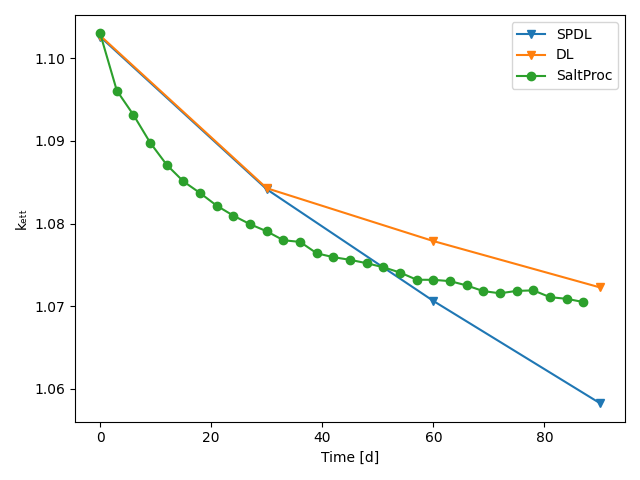
\includegraphics[scale=0.5]{images/soln-1-keff.png}
  \caption{k$_{eff}$ over time comparing steady batchwise results to continuous methods.}
   \label{fig:steady-compare-keff}
\end{figure}

\begin{figure}[H]
  \centering
  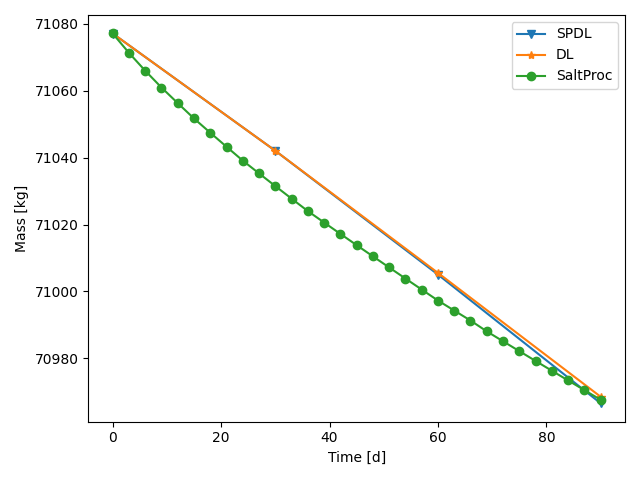
\includegraphics[scale=0.5]{images/soln-1-th232.png}
  \caption{Thorium-232 mass over time comparing steady batchwise results to continuous methods.}
   \label{fig:steady-compare-th232}
\end{figure}

The uranium-233 mass over time for the different methods reflects very closely with the effective multiplication factors. The uranium-233 comes from beta decay of protactinium-233, where protactinium is one of the elements designated to be removed in the MSBR reprocessing scheme. For Direct Linear, the removal of protactinium is approximated using 100\% removal over three days. For SaltProc Direct Linear, the removal is instead approximated to 9.5\% over 3 days, which is the value used in steady SaltProc. However, because the SPDL method is continuously removing the protactinium, this means that there is less protactinium-233 which decays into uranium-233 when compared to the steady batchwise method in SaltProc. 

\begin{figure}[H]
  \centering
  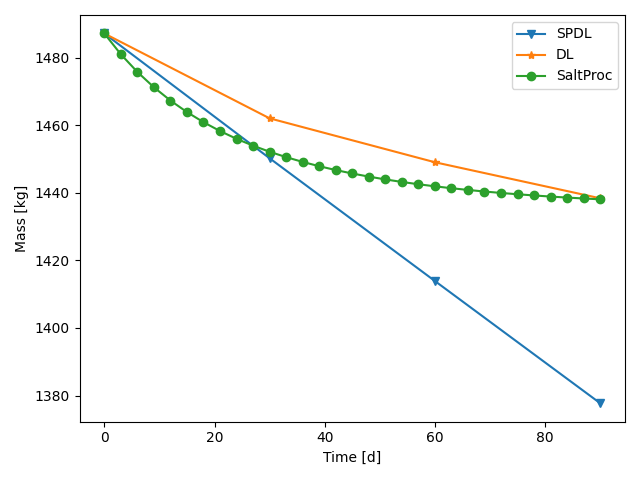
\includegraphics[scale=0.5]{images/soln-1-u233.png}
  \caption{Uranium-233 mass over time comparing steady batchwise results to continuous methods.}
   \label{fig:steady-compare-u233}
\end{figure}

A similar effect with the protactinium can be seen in Figures \ref{fig:steady-compare-xe135} and \ref{fig:steady-compare-xe136}. Although the SPDL method is using a reprocessing constant which should allow for matching SaltProc, the continuous removal results in fairly large discrepancies. The xenon-135 difference is only on the order of tenths of a gram, but because the quantity is constantly suppressed in the continuous SPDL method, the overall capture is reduced drastically, resulting in a difference of roughly 40 grams in the xenon-136 mass.

\begin{figure}[H]
  \centering
  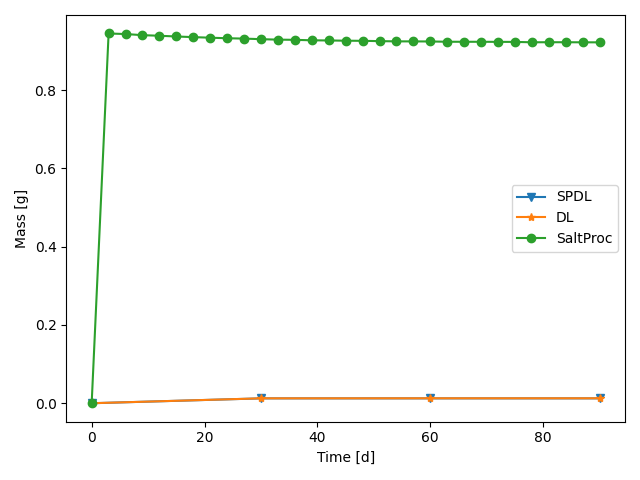
\includegraphics[scale=0.5]{images/soln-1-xe135.png}
  \caption{Xenon-135 mass over time comparing steady batchwise results to continuous methods.}
   \label{fig:steady-compare-xe135}
\end{figure}

\begin{figure}[H]
  \centering
  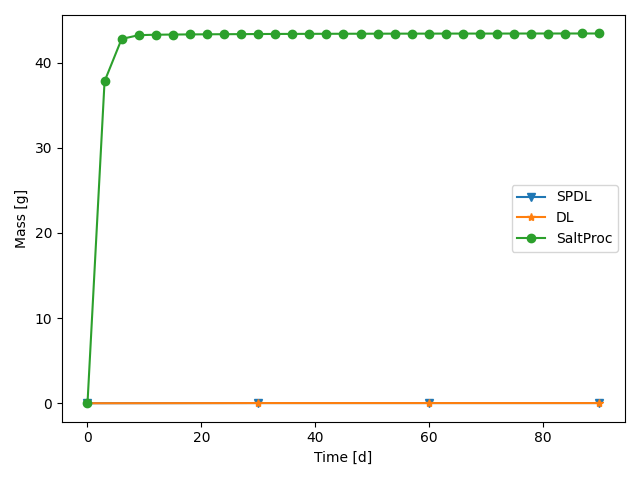
\includegraphics[scale=0.5]{images/soln-1-xe136.png}
  \caption{Xenon-136 mass over time comparing steady batchwise results to continuous methods.}
   \label{fig:steady-compare-xe136}
\end{figure}

Overall, using a continuous method to approximate a steady batchwise method does not seem generally viable. This is because isotopes which are continuously removed have a very different behaviour from isotopes which are removed after interactions occur over an entire depletion step. If the reprocessing scheme calls for a batchwise process, it may be important to reactor behaviour to allow for those capture or decay processes to occur without influence from reprocessing.

\subsection{Overall Differences}

Figures \ref{fig:prev-cur-keff-plot} through  \ref{fig:prev-cur-xe136-plot} show how the previous work, using a steady batchwise reprocessing method with the average uranium-233 feed, and the current work, using the direct linear continuous method with the realistic protactinium decay, compare with each other. The previous work uses the long term bulk average uranium-233 feed rate, and implements altered cycle rates for protactinium, xenon, and krypton. The continuous method uses only the cycle time data from the Robertson report to generate the reprocessing constants \cite{robertson_conceptual_1971}.

The effective multiplication factor for the two different approaches initially has the previous work falling faster. This is due to the initial buildup of fission product poisons, while the continuous reprocessing allows for these poisons to be removed more efficiently. However, as time goes on, the lacking uranium-233 feed due to the empty protactinium decay tank causes the current work to dip below the previous work. Over the course of three months, the longer lived behaviour cannot be seen. However, the section covering the advanced protactinium decay model in more depth shows the results over the course of several years and reveals that the reactivity difference due to the different refueling methods eventually decreases.

\begin{figure}[H]
  \centering
  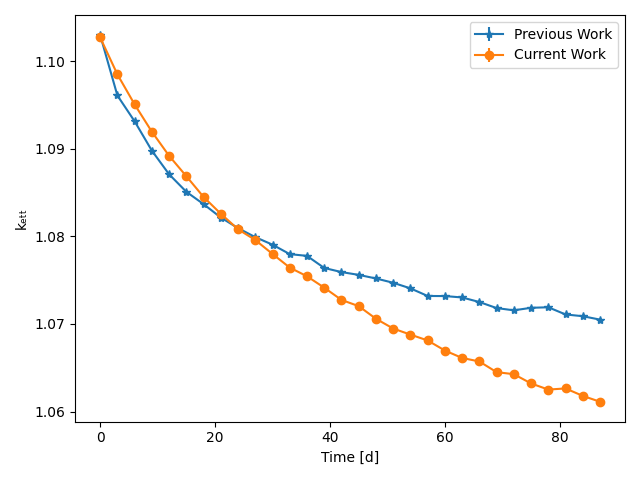
\includegraphics[scale=0.5]{images/prev-cur-keff.png}
  \caption{k$_{eff}$ over time with three day depletion steps for steady batchwise and Direct Linear continuous reprocessing using different uranium-233 feed schemes.}
   \label{fig:prev-cur-keff-plot}
\end{figure}

The thorium-232 feed rate for both approaches is the same, yet the previous work burns it slightly faster than the current work. This effect is likely caused by the presense of more uranium-233 in the previous work, which allows for a faster burn rate of the thorium-233 due to a higher net flux.

\begin{figure}[H]
  \centering
  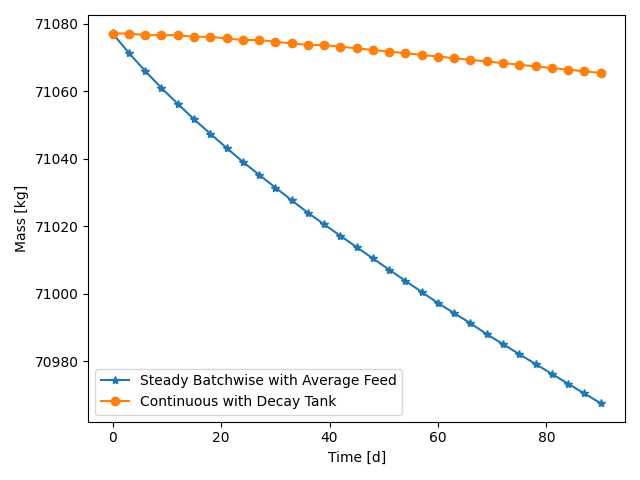
\includegraphics[scale=0.5]{images/prev-cur-th232.png}
  \caption{\ce{^{232}Th} over time with three day depletion steps for steady batchwise and Direct Linear continuous reprocessing using different uranium-233 feed schemes.}
   \label{fig:prev-cur-th232-plot}
\end{figure}

This difference in the uranium-233 masses is primarily due to the effects of the different uranium-233 feed rate approaches implemented in each of the different works.

\begin{figure}[H]
  \centering
  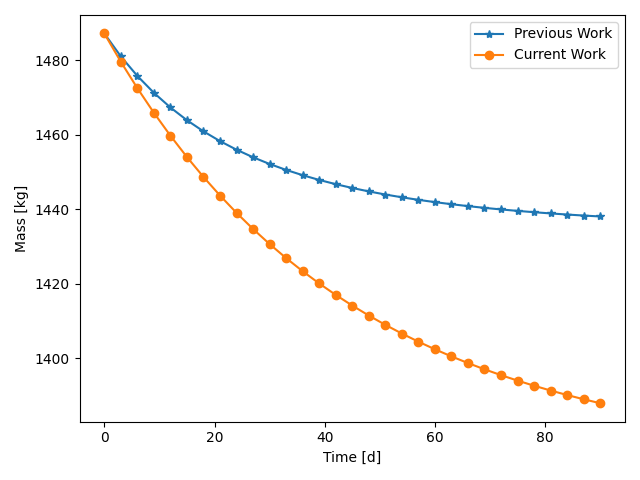
\includegraphics[scale=0.5]{images/prev-cur-u233.png}
  \caption{\ce{^{233}U} over time with three day depletion steps for steady batchwise and Direct Linear continuous reprocessing using different uranium-233 feed schemes.}
   \label{fig:prev-cur-u233-plot}
\end{figure}

For the xenon-135 and xenon-136, these results are primarily impacted due to the continuous and reprocessing methods implemented. 

\begin{figure}[H]
  \centering
  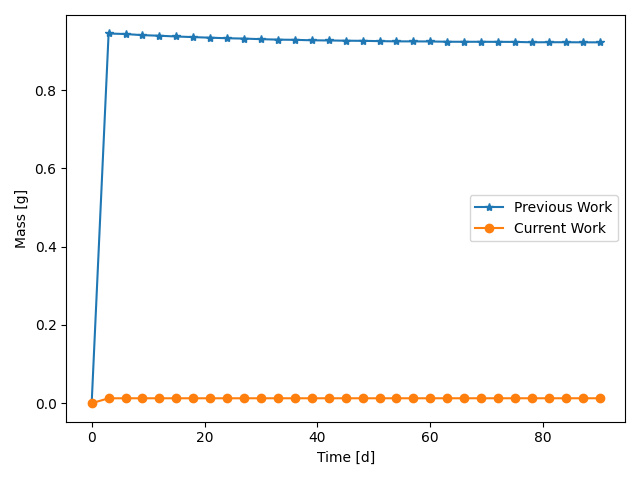
\includegraphics[scale=0.5]{images/prev-cur-xe135.png}
  \caption{\ce{^{135}Xe} over time three day depletion steps for steady batchwise and Direct Linear continuous reprocessing using different uranium-233 feed schemes.}
   \label{fig:prev-cur-xe135-plot}
\end{figure}

\begin{figure}[H]
  \centering
  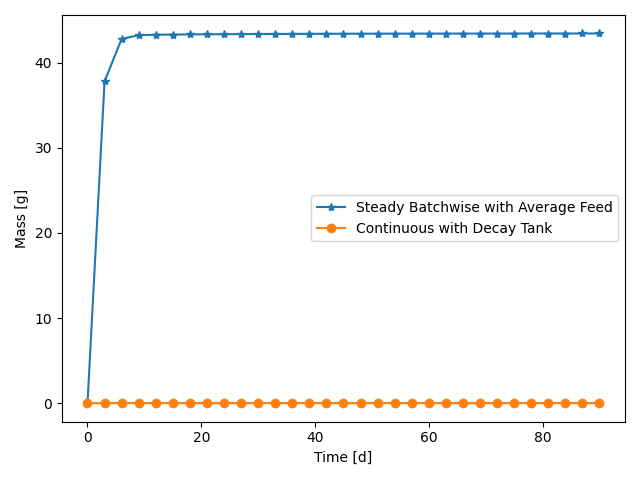
\includegraphics[scale=0.5]{images/prev-cur-xe136.png}
  \caption{\ce{^{136}Xe} over time three day depletion steps for steady batchwise and Direct Linear continuous reprocessing using different uranium-233 feed schemes.}
   \label{fig:prev-cur-xe136-plot}
\end{figure}

Overall, these results show the combined effects of implementing continuous reprocessing methods with a continuously updated uranium-233 refeed tank which is initially empty. This is compared with batchwise reprocessing methods and an averaged uranium-233 feed rate.

%\subsection{One Year Depletion}

%The results of a one year net depletion time can be seen in Figures \ref{fig:optimal-compare-sspdldl-2}  through \ref{fig:SPCR-cont-136Xe-2}, which reflect the results shown in Figures \ref{fig:optimal-compare-sspdldl}  through \ref{fig:SPCR-cont-136Xe}.

%\begin{figure}[H]
%  \centering
%  
\includegraphics[scale=0.1]{images/placeholder.png}
%  \caption{k$_{eff}$ over time with small depletion steps for steady batchwise, SaltProc Direct Linear continuous, and Direct Linear continuous reprocessing.}
%   \label{fig:optimal-compare-sspdldl-2}
%\end{figure}

%\begin{figure}[H]
%  \centering
%  
\includegraphics[scale=0.1]{images/placeholder.png}
%  \caption{\ce{^{235}U} over time with small depletion steps for steady batchwise, SaltProc Direct Linear continuous, and Direct Linear continuous reprocessing.}
%   \label{fig:SPCR-cont-235u-2}
%\end{figure}

%\begin{figure}[H]
%  \centering
%  
\includegraphics[scale=0.1]{images/placeholder.png}
%  \caption{\ce{^{135}Xe} over time with small depletion steps for steady batchwise, SaltProc Direct Linear continuous, and Direct Linear continuous reprocessing.}
%   \label{fig:SPCR-cont-135Xe-2}
%\end{figure}

%\begin{figure}[H]
%  \centering
  %
\includegraphics[scale=0.1]{images/placeholder.png}
%  \caption{\ce{^{136}Xe} over time with small depletion steps for steady batchwise, SaltProc Direct Linear continuous, and Direct Linear continuous reprocessing.}
%   \label{fig:SPCR-cont-136Xe-2}
%\end{figure}

%\subsection{Ten Year Depletion}

%CONTINUOUS AND BULK SALTPROC PREVIOUS RESULTS \hline

%The results of a one year net depletion time can be seen in Figures \ref{fig:optimal-compare-sspdldl-2}  through \ref{fig:SPCR-cont-136Xe-2}, which reflect the results shown in Figures \ref{fig:optimal-compare-sspdldl}  through \ref{fig:SPCR-cont-136Xe}.

%\begin{figure}[H]
%  \centering
%  
\includegraphics[scale=0.1]{images/placeholder.png}
%  \caption{k$_{eff}$ over time with small depletion steps for steady batchwise, SaltProc Direct Linear continuous, and Direct Linear continuous reprocessing.}
%   \label{fig:optimal-compare-sspdldl-2}
%\end{figure}

%\begin{figure}[H]
%  \centering
%  
\includegraphics[scale=0.1]{images/placeholder.png}
%  \caption{\ce{^{235}U} over time with small depletion steps for steady batchwise, SaltProc Direct Linear continuous, and Direct Linear continuous reprocessing.}
%   \label{fig:SPCR-cont-235u-2}
%\end{figure}

%\begin{figure}[H]
%  \centering
%  
\includegraphics[scale=0.1]{images/placeholder.png}
%  \caption{\ce{^{135}Xe} over time with small depletion steps for steady batchwise, SaltProc Direct Linear continuous, and Direct Linear continuous reprocessing.}
%   \label{fig:SPCR-cont-135Xe-2}
%\end{figure}

%\begin{figure}[H]
%  \centering
%  
\includegraphics[scale=0.1]{images/placeholder.png}
%  \caption{\ce{^{136}Xe} over time with small depletion steps for steady batchwise, SaltProc Direct Linear continuous, and Direct Linear continuous reprocessing.}
%   \label{fig:SPCR-cont-136Xe-2}
%\end{figure}


\section{Mass Balancing}

The continuous reprocessing method allows for larger depletion steps to be used without losing out on the impact of reprocessing while also allowing for fewer simulations to be run when compared to batchwise methods. However, one potential issue which is possible for continuous methods but not typically an issue for batchwise methods is mass balancing. 

The effects of mass balancing are of particular note in the Serpent2 code because an increase in mass causes a corresponding increase in density due to constant volumes. A simple workaround to this is to either remove some fraction of mass to return the net mass to equilibrium or adjust the volumes so the density remains constant, thus maintaining physicality.

However, if the issue of mass balancing is not considered, then the results could be fairly inaccurate, potentially without anyone noticing. This is because changes in isotopic composition and densities are expected. The issue comes about when these changes are caused by adding more material to a space than is physically possible, thus generating non-physical results.

\subsection{Impact Minimization Using Modified Feeds}

One aspect investigated is minimizing the change in the net mass by only altering the average feed rates implemented. It is determined through repeated simulations that increasing the thorium-2323 feed rate drives the second derivative of the net mass negative. The uranium-233 feed increasing drives the second derivative to be positive. The reason for these effects are due to the change in the effective multiplication factor, mass of the added feed, and removal of fission products by reprocessing.

Using these relationships, a process to determine the feed rates to minimize the change in the net mass is determined. The process is as follows:  hold one feed rate constant while adjusting the other;
if the final net mass is higher than initial net mass, then reduce the feed rates and vice versa;
once the final net mass is same as initial net mass, make adjustment based on second derivative;
if the second derivative is positive, increase thorium-232 or decrease uranium-233 feed;
if the second derivative is negative, increase uranium-233 or decrease thorium-232 feed;
iterate until second derivative is zero and net mass remains roughly constant.

After iterating through this processes several times using a depletion time step of 300 days over 10 steps, the modified average feed rates of 1.9 kg/day of thorium-232 and 2.16 kg/day of uranium-233 were determined to result in a very small change to the net mass on the order of 0.02\%.

\subsection{Actual Impact}

Previously, the maximum impact of improper mass balancing was calculated and was shown to have a 21\% difference impact on the density of thorium-232. However, it is expected for the thorium-232 mass to change over time, so only viewing the mass of thorium is not very useful. Instead, viewing the net mass of the system will allow for insight into how the overall system behaviour could be expected to change due to density variations.

\begin{figure}[H]
  \centering
  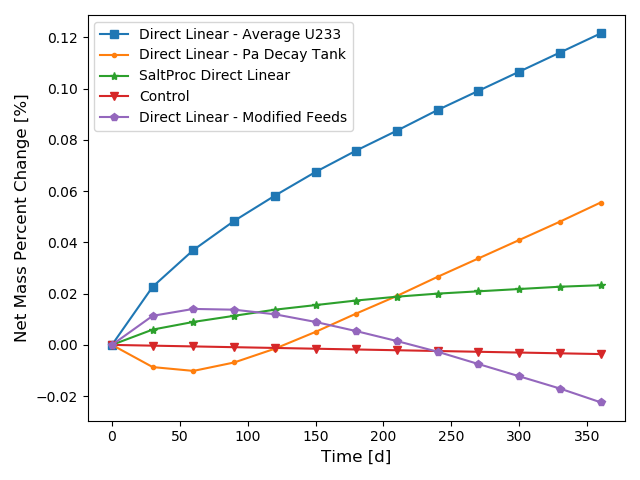
\includegraphics[scale=0.5]{images/net-mass-pcnt-change.png}
  \caption{Change in net mass of the fuel salt for various methods.}
   \label{fig:net-mass-bal}
\end{figure}

Figure \ref{fig:net-mass-bal} shows the evolution of the net mass of the fuel salt over time while using a 30 day depletion time step over 360 days. The method which has the largest change in the net mass is the Direct Linear method with the averaged uranium-233 feed rate. The net mass difference is roughly 198 kilograms, which appears to be fairly substantial. However, the approximate impact upon the simulation accuracy is dependent on the density. Equation \eqref{eq:new_rho_2} shows how the final density is impacted by the added mass, where the initial fuel salt density, $\rho_0$, is 3.35 grams per cubic centimeter. 

\begin{equation} \hfill
\rho_f = \frac{m_0 + \Delta m}{V} = \rho_0 + \Delta \rho
\hfill\label{eq:new_rho_2} \end{equation}

Continuing with the Direct Linear case using the averaged uranium-233 feed, the change in the density is on the order of four milligrams per cubic centimeter, yielding a final density percent difference of 0.12\%. In terms of the impact on overall results, the change in density due to implementing the continuous method is fairly negligible unless the required simulation is of very high precision.

%\subsection{Magnified Impact}

%One target parameter which could be optimized is the change in the net mass of the core over depletion in order to minimize effects of mass imbalance.

%2D TABLES FOR DIFFERENT U-233 AND TH-232 FEED RATES (th-232 masses, u-233 masses, etc.)

%\section{Isotopic Development}

%USING STEPS PREVIOUSLY DETERMINED, COMPARE WITH ANDREI'S THESIS USING CONTINUOUS METHODS.

%\section{Neutronic Parameters}

%GENERATED ALONG WITH ISOTOPIC DEVELOPMENT (Check Andrei's thesis, include spectra, feedback coeffs, etc. for BOC and SS).

%\subsection{Feed Rate Perturbation}

